
%%% Local Variables:
%%% TeX-command-extra-options: "-shell-escape"
%%% mode: latex
%%% TeX-master: t
%%% End:
\documentclass{beamer}
\usepackage{caption}
\usepackage{minted}
\usepackage[labelformat=simple]{subcaption}

\usetheme{Singapore}
\title{Lecture 2}
%\subtitle{in Racket}
%\author{Peter Campora}
%\institute{ULL}
%\date{\today}

%This lectures introduces Dr. Racket and the wrong way to program
\begin{document}
\begin{frame}
\titlepage
\end{frame}

\section{Intro}

\begin{frame}
  \frametitle{Dr. Racket}
  \begin{columns}
    \column{0.45\textwidth}
    I encourage the use of Dr. Racket:
    \begin{itemize}
    \item<1-> The definitions window (top) is for writing programs
    \item<2-> The interactions window (bottom) is for interaction
    \item<3-> Let me demonstrate 
    \end{itemize}
    \column{0.45\textwidth}
    \begin{figure}
      \centering 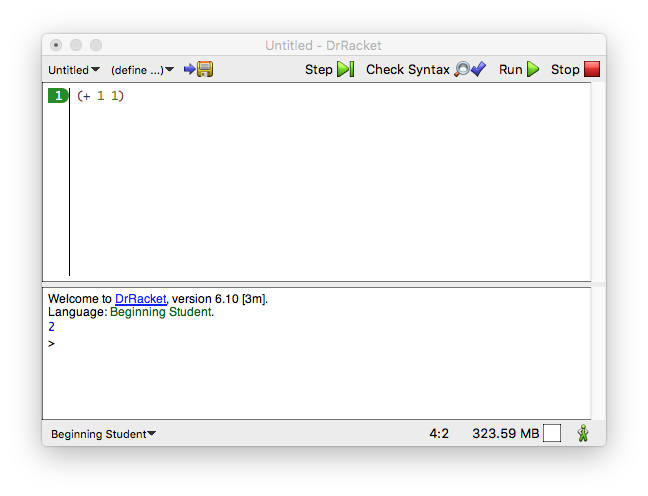
\includegraphics[width=0.9\textwidth]{images/drracket-plain.png}
    \end{figure}
  \end{columns}
\end{frame}

\begin{frame}
  \frametitle{Relevant XKCDs}
  \begin{figure}
    \centering 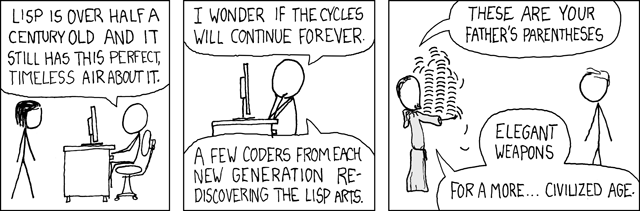
\includegraphics[width=0.8\textwidth]{images/lisp_cycles.png}
  \end{figure}    
  % 
  \begin{figure}
    \centering 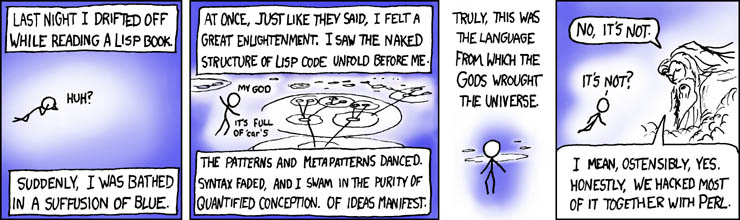
\includegraphics[width=0.8\textwidth]{images/lisp.jpg}
  \end{figure}    
\end{frame}

% \defverbatim[colored]\lstR{
% \begin{minted}{Scheme}
% ;;Number -> Number
% (define (square x) (* x x))

% ;;Number List -> Number List
% (define (sum-of-squares lst)
%   (sum (map square lst))         
% \end{minted}
% }

\defverbatim[colored]\syntaxOne{
\begin{minted}{Scheme} 
    (f 1)  
\end{minted}
}

\defverbatim[colored]\syntaxTwo{
\begin{minted}{Scheme} 
    (+ 1 2)
\end{minted}
}

\defverbatim[colored]\syntaxThree{
\begin{minted}{Scheme} 
    (+ 1 (* 2 3))
\end{minted}
}

\defverbatim[colored]\syntaxFour{
\begin{minted}{Scheme} 
    (define (double x) (* x 2))
\end{minted}
}

\section{Syntax}
\begin{frame}
  \frametitle{Syntax Primer}
  Functional Programming is about \emph{functions}
  \begin{itemize}
  \item<1-> To call a function f, with argument 1 we write: \syntaxOne
  \item<2-> Instead of 1+2 we write: \syntaxTwo
  \item<3-> There is no operator precedence. 1 + 2*3 becomes: \syntaxThree
  \item<4-> To define a function that doubles numbers: \syntaxFour    
  \end{itemize}
\end{frame}

\begin{frame}
  \frametitle{Ewww Gross Syntax!}
  \begin{center}
    \includegraphics[width=0.45\textwidth]{images/syntax-yoda.jpg}
    \begin{itemize}
    \item<2-> Racket (Lisps in general) use prefix (polish) notation
    \item<3-> Tons of advantages:
      \begin{enumerate}
      \item<4-> Easy to fit the grammar in your head (unlike C++)
      \item<5-> Racket is \emph{homoiconic}
      \item<6-> Makes the language extensible
      \item<7-> Allows for structured editing
      \end{enumerate}
    \item<8-> However one large disadvantage is that it is \emph{different}
    \item<9-> You'll get used to it
    \end{itemize}
  \end{center}
\end{frame}


\section{First Program}
\begin{frame}
  \frametitle{Let's Write a Program!}
  We're going to write a program to make a rocket land, SpaceX style.
  \begin{center}
    \includegraphics[width=0.3\textwidth]{images/SpaceX.jpg}
  \end{center}
  \begin{itemize}
  \item<2-> First, let's post an image of a rocket into Dr. Racket
  \item<3-> \includegraphics[width=0.05\textwidth]{images/rocket.png}
  \item<4-> \includegraphics[width=0.4\textwidth]{images/rocket-in-interactions.png}
  %\item<4-> \includegraphics[width=0.3\textwidth]{images/function-image.png}
  \end{itemize}
\end{frame}

\defverbatim[colored]\rocketSize{
\begin{minted}{Scheme} 
  (define rocket-size 
    (* (image-width rocket) (image-height rocket)))
\end{minted}
}

\defverbatim[colored]\circle{
\begin{minted}{Scheme} 
(circle 20 "solid" "red")
\end{minted}
}

\defverbatim[colored]\rectangle{
\begin{minted}{Scheme} 
(rectangle 30  20 "outline" "blue")
\end{minted}
}

\begin{frame}
  \frametitle{Messing With Images}
  Let's play around with our rocket:
  \begin{itemize}
  \item \includegraphics[width=0.4\textwidth]{images/define-rocket.png}
  \item<2-> Now let's create a function to calculate its size:
  \item[]<3-> \rocketSize
  \item<4-> We can define circles: \mintinline{Scheme}{(circle 20 "solid" "red")}
  \item<4-> Or rectangles: \mintinline{Scheme}{(rectangle 30  20 "outline" "blue")}
  \end{itemize}
\end{frame}

\defverbatim[colored]\emptyScene{
\begin{minted}{Scheme} 
  (empty-scene 100 100)
\end{minted}
}

\defverbatim[colored]\initialScene{
\begin{minted}{Scheme} 
  (place-image (circle 10 "solid" "green")
             50 80
             (empty-scene 100 100))
\end{minted}
}

\begin{frame}
  \frametitle{Drawing a Scene}
  We'll start by drawing an empty scene.
  \begin{itemize}
  \item \mintinline{Scheme}{(empty-scene 100 100)}
  \item<2-> \emph{Boring!} Let's add something to it:
  \item[]<3-> \initialScene
  \item<4->Here's what our new scene looks like: \includegraphics[width=0.1\textwidth]{images/initial-scene.png}
  \end{itemize}
\end{frame}

\defverbatim[colored]\placeRocket{
\begin{minted}{Scheme} 
  (place-image rocket 50 20 (empty-scene 100 60))
\end{minted}
}

\begin{frame}
  \frametitle{Rocket Fun}
  Let's consider placing the rocket in the scene:
  \begin{itemize}
  \item<2->[] \placeRocket
  \item<3-> \includegraphics[width=0.1\textwidth]{images/placed_rocket.png}
  \item<4-> Let's open Dr. Racket and try moving the rocket up and down.
  \item<5-> As you can see, higher numbers for y move it lower
  \end{itemize}
\end{frame}

% \begin{frame}
%   \frametitle{Moving Rockets}
%   So, let's try to move the rocket from top to bottom.
%   \begin{itemize}
%   \item \placeRocket
%   \item<1-> \includegraphics[width=0.1\textwidth]{images/placed-rocket.png}
%   \item<2-> Let's open Dr. Racket and try moving the rocket up and down.
%   \item<3-> As you can see, higher numbers for y move it lower.
%   \end{itemize}
% \end{frame}

\defverbatim[colored]\placeRocket{
\begin{minted}{Scheme} 
  (define (picture-of-rocket height)
    (place-image  50 height (empty-scene 100 60)))
\end{minted}
}

\defverbatim[colored]\animate{
\begin{minted}{Scheme} 
  (animate picture-of-rocket)
\end{minted}
}

\begin{frame}
  \frametitle{Baby's First Animation}
  Here's a first attempt at a function that places the rocket at a height.
  \begin{itemize}
  \item \placeRocket
  \item<2-> Now let's mess with the \emph{animate} function
  \item<3-> \mintinline{Scheme}{(animate picture-of-rocket)}
  \item<4-> Anything weird about this expression?
  \item<5-> This is our first example of using \emph{higher-order} function,
    a function that takes another function as input or produces another function
    as output.
  \item<6-> One example of a famous higher order function is $\frac{d}{dx}$
  \end{itemize}
\end{frame}

\defverbatim[colored]\sign{
\begin{minted}{Scheme}
  (define (sign x)
    (cond
      [(< x 0) -1]
      [(> x 0) 1]
      [else 0]))
\end{minted}
}

\defverbatim[colored]\signJava{
\begin{minted}{Java}
  public int sign(int x) {
    if (x < 0)
      return -1
    else if (x > 0)
      return 1
    else 
      return 0
  }
\end{minted}
}

\section{Refactoring}
\begin{frame}
  \frametitle{Was Our Animation Good?}
  \begin{itemize}
  \item<1-> It wasn't so nice that our rocket flew through the ground
  \item<2-> So let's fix that.
  \item<3-> First, we need to introduce conditional expressions:
  %\item<4-> Let's consider the sign function
  \item<4-> \sign
  \item<5-> \signJava
  \end{itemize}
\end{frame}

\defverbatim[colored]\versionTwo{
\begin{minted}{Scheme}
(define (picture-of-rocket.v2 height)
  (cond 
    [(<= height 60) 
      (place-image rocket 50 height (empty-scene 100 60))]
    [else 
      (place-image rocket 50 60 (empty-scene 100 60))]))
\end{minted}
}

\begin{frame}
  \frametitle{Fix the Landing}
  Let's try out a new version of the function:
  \begin{itemize}
  \item<2-> \versionTwo
  \item<3-> Is there anything wrong with this code?
    \begin{enumerate}
    \item<4-> Magic numbers
    \item<5-> Repeated empty-scene call
    \end{enumerate}
  \item<6-> What about the landing?
  \item<7-> Let's clean it up a bit.
  \end{itemize}
\end{frame}

\defverbatim[colored]\rocketCenter{
\begin{minted}{Scheme}
  (define rocket-center-to-top 
    (- canvas-height (/ rocket-height 2)))
\end{minted}
}

\begin{frame}
  \frametitle{Fix the Landing (cont)}
  The landing should take into account the midpoint of the rocket and the canvas-height.
  \begin{itemize}
  \item<1-> No more magic numbers!
  \item<2-> \mintinline{Scheme}{(define canvas-height 60)}
  \item<3-> Now let's get the center point:
  \item<4-> \rocketCenter
  \item<5-> Let's look at our new version.
  \end{itemize}
\end{frame}

\defverbatim[colored]\rocketThree{
\begin{minted}[fontsize=\footnotesize]{Scheme}
(define (picture-of-rocket.v3 height)
  (cond
    [(<= height rocket-center-to-top) 
      (place-image rocket canvas-mid-width height canvas)]
    [else
      (place-image rocket canvas-mid-width rocket-center-to-top canvas)]))
\end{minted}
}

      
\defverbatim[colored]\rockBed{
\begin{minted}{Scheme}
  (define rock-bed
    (rectangle canvas-width 10 "solid" "grey"))
\end{minted}
}
\defverbatim[colored]\blueCanvas{
\begin{minted}{Scheme}
  (define blue-canvas 
    (empty-scene canvas-width canvas-height "blue"))
\end{minted}
}
      
\begin{frame}
  \frametitle{Good Now?}
  \rocketThree
  \begin{itemize}
  \item<1-> Looks a lot better to me, in animation and code.
  \item<2-> It's a bit weird that it lands on ``nothing'', so let's add a rock bed and a blue background.
  \item<3-> \rockBed
  \item<4-> \blueCanvas
  \end{itemize}
\end{frame}

\defverbatim[colored]\versionFour{
\begin{minted}[fontsize=\footnotesize]{Scheme}
(define (picture-of-rocket.v4 height)
  (cond
   [(<= height rocket-center-to-top) 
    (place-image rocket canvas-mid-width height
      (place-image rock-bed canvas-mid-width canvas-height blue-canvas))]
   [else
    (place-image rocket canvas-mid-width rocket-center-to-top 
      (place-image rock-bed canvas-mid-width canvas-height blue-canvas))]))
\end{minted}
}

\begin{frame}
  \frametitle{Rockbedding and Rolling}
  \versionFour
  \pause
  \begin{center}
    \includegraphics[width=0.2\textwidth]{images/dora.jpeg}
  \end{center}
\end{frame}

\begin{frame}
  \frametitle{But do We Understand Animate?}
  Let's look up what exactly it does in the online documentation.
  \begin{itemize}
  \item<1-> \url{https://docs.racket-lang.org/teachpack/2htdpuniverse.html}
  \item<2-> So, animate applies the argument function with a \emph{time} that
    is used to create an image.
  \item<3-> Does our code have a big problem then?
  \item<4-> We are using time as distance!
  \item<5-> We need one last version of the program.
  \end{itemize}
\end{frame}

\defverbatim[colored]\velocity{
\begin{minted}[fontsize=\footnotesize]{Scheme}
(define velocity 3)
\end{minted}
}

\defverbatim[colored]\distance{
\begin{minted}[fontsize=\footnotesize]{Scheme}
;;move at three units per second
(define (distance time) (* time velocity))
\end{minted}
}

\defverbatim[colored]\versionFive{
\begin{minted}[fontsize=\footnotesize]{Scheme}
(define (picture-of-rocket.v5 time)
  (cond
   ((<= (distance time) rocket-center-to-top) 
    (place-image rocket canvas-mid-width (distance time) 
     (place-image rock-bed canvas-mid-width canvas-height blue-canvas)))
   (else
    (place-image rocket canvas-mid-width rocket-center-to-top 
     (place-image rock-bed canvas-mid-width canvas-height blue-canvas)))))
\end{minted}
}

\begin{frame}
  \frametitle{Last Fix}
  Fix:
  \begin{enumerate}
  \item<1-> \mintinline{Scheme}{(define velocity 3)}
  \item<2-> \mintinline{Scheme}{(define (distance time) (* time velocity))}
  \end{enumerate}
  \pause
  \versionFive
\end{frame}

\section{Are We Functional Programmers Now?}
\begin{frame}
  \frametitle{Congratulations!}
  You're a functional programmer now! ...
  \begin{itemize}
  \item<1-> Right?
  \item<2-> Of course not!
  \item<3-> Many other courses might try to continue introducing features in this manner...
  \item<4-> But this lecture was messy and barely motivated the need for novel
    things like higher order functions, that I glossed over.
  \item<5-> So, next lecture we're going to \emph{slow down} and take a systematic
    approach.
  \end{itemize}
\end{frame}

\begin{frame}
  \frametitle{A Glimpse of the Future}
  \begin{center}
    \includegraphics[width=0.4\textwidth]{images/design-recipes.png}
  \end{center}
  \begin{itemize}
  \item We'll start with a slow paced introduction to the basic building blocks
    of programs.
  \item Then we'll move onto how to create and call functions.
  \item Then we'll discuss the two fundamental kinds of programs, batch programs
    (scripts) and big bang programs (event driven).
  \item Then finally, how to \emph{design} these kinds of programs.
  \end{itemize}
\end{frame}

\end{document}
%%% Local Variables:
%%% mode: latex
%%% TeX-master: t
%%% End:
